\chapter{SSH}
SSH, or Secure Shell, is a network protocol that allows for secure
communication between two computers. It has been introduced in 1995 by
Tatu Ylönen, a Finnish computer scientist, but has been since
commercialized so it was not open source anymore. A open source fork 
called OpenSSH has been created and is now the most used
implementation of SSH. Nowadays is the most widely diffused version of 
SSH and is the one we will refer to in this document.

\begin{boxH}
  Here we will always refer to SSH-2 (unless otherwise noted)
\end{boxH}

\section{Architecture}
SSH is a three layer architecture, which sits on top of TLS, which as
alway provides initial connection, server authentication,
confidentiality and integrity and key re-exchange (RFC-4253 recommends
after 1GB of data transmitted or after 1 hour of transmission) which
is crucial for long running connections.\\
there is also a specific protocol for user authentication, and a
connection protocol too, which supports supports multiple connections
(channels) over a single secure channel (implemented with the
transport layer protocol). This means that SSH can as as a
site-to-site VPN.
\subsection{SSH Transport Layer Protocol}
The connection is setup with TCP, by default on port 22, on which the
client initiates the connection.\\
Then the SSH version string is exchanges, which contains the security
features supported. Both sides must send a version string of the
following form: SSH-protoversion-softwareversion SP comments CR LF.
Its also used to triggers compatibility extensions.\\
All packets that follow the version string exchange is sent using the
Binary Packet Protocol. Then the keys are exchanged, at which point
the data can be exchanged and then the connection is closed.
\begin{figure}[H]
  \centering
  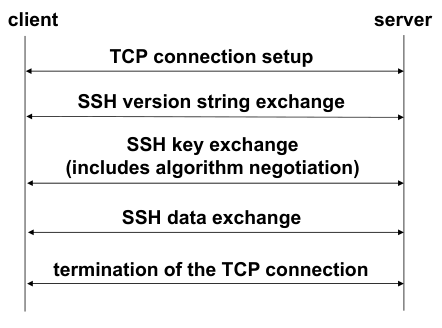
\includegraphics[width=.6\textwidth]{img/SSH layer protocol.png}
  \caption{SSH Transport Layer Protocol}
\end{figure}
\subsubsection{Binary Packet Protocol}
\begin{figure}[H]
  \centering
  \includegraphics[width=.6\textwidth]{img/SSH bynary packet
  protocol.png}
  \caption{Binary Packet Protocol}
\end{figure}
The Binary Packet Protocol is pretty simple, it consists of:
\begin{itemize}
  \item the length of the packet (4 bytes), which does not include the
    MAC and the packet length field itself
  \item the payload, which may be compressed. Its size is the length
    of the packet minus the length of the length field minus 1 (for
    the padding length field), up to a maximum uncompressed size of
    32768 bytes(32KB)
  \item the random padding
  \item the MAC
\end{itemize}

By default the communication is in binary.

\subsubsection{key exchange}
\subsubsection{Algorithm specification}
\subsubsection{Diffie-Hellman key exchange}
This is also an implicit authentication of the server.\\
In this phase the client generates a random number $x$ and computes
$e=g^x \mod p$ and sends it to the server. The server generates a
random number $y$ and computes $f=g^y \mod p$ and sends it to the
client. The server computes $K=e^y \mod p$ and exchange
$H=\text{HASH}(K)$. The server generates the signature on $H$ using
its private key and sends 

\subsubsection{key derivation}
Many keyed digest require a initialization vector

session\_id is the hash value computed for the first key 
exchange, and remains such even when key re-exchange is 
performed
\subsubsection{Encryption}
The supported algorithms are:
\begin{itemize}
  \item (required) 3des-cbc (w/ three keys, i.e. 168 bit key)
  \item(recommended) aes128-cbc
  \item(optional) blowfish-cbc, twofish256-cbc, twofish192-cbc,
    twofish128-cbc, aes256-cbc, aes192-cbc, serpent256-cbc,
    serpent192-cbc, serpent128-cbc, arcfour, idea-cbc, cast128-cbc,
    none
\end{itemize}

\subsubsection{MAC}
